\subsection{Язык \logiql}
\label{sec:technology:logiql}

\subsubsection{Определение предикатов}
\label{sec:technology:logiql:predicates}

Для более наглядного представления об этом языке следует разобрать пример из предыдущей главы.

\begin{lstlisting}[language=Prolog]
sales_u(product, store, day, unit) ->
  string(product),
  string(store),
  datetime(day),
  int(units).
\end{lstlisting}

Или, аналог \sql:

\begin{lstlisting}[language=SQL]
CREATE TABLE sales_u
(
  product VARCHAR(15) NOT NULL,
  store VARCHAR(20) NOT NULL,
  day DATETIME NOT NULL,
  unit INT NOT NULL
);
\end{lstlisting}

Здесь \lstinline{sales_u} является предикатом - аналог термина «таблица» в
\sql. Из записи видно, что этот предикат состоит из 4 колонок, типы которых \lstinline{string}, \lstinline{string}, \lstinline{datetime}, \lstinline{int} соответственно. Если быть точнее, то определение должно быть дано немного другим образом: если в предикате \lstinline{sales_u} есть некоторая запись, то это означает, что тип значения в первой колонке должен быть \lstinline{string}, второй – \lstinline{string}, третьей – \lstinline{datetime}, и, наконец, четвертой – \lstinline{int}. Об этом свидетельствует знак импликации (\lstinline{->}). При этом стоит отметить, что здесь важен лишь порядок следования значений в предикате, \lstinline{product}, \lstinline{store}, \lstinline{day}, \lstinline{units} – это лишь псевдонимы значений на этих позициях в данном контексте. Это, как упоминалось ранее, определение схемы.

\subsubsection{Жизненный цикл транзакции}
\label{sec:technology:logiql:transaction}

Как и язык \sql, \logiql имеет свой жизненный цикл транзакций. Согласно Википедии \cite{transaction_definition} транзакция – группа последовательных операций с базой данных, которая представляет собой логическую единицу работы с данными. Транзакция может быть выполнена целиком и успешно, соблюдая целостность данных и независимо от параллельно идущих других транзакций, либо не выполнена вообще, и тогда она не должна произвести никакого эффекта.
В \logiql также имеется понятие \emph{workspace} (рабочее пространство) – своеобразное пространство имен, хранилище для особых предикатов. В этом пространстве содержатся как данные, так и программный код, который был либо был написан разработчиком, либо сгенерирован системой. Рисунок \ref{fig:technology:logiql:transaction} показывает упрощенную версию жизненного цикла этого пространства \cite{query_language_for_smart_db}.
Изначально надо создать \emph{workspace}. Изначально он будет содержать только стандартный набор системных предикатов. Созданный \emph{workspace} можно изменять через транзакции.
Чтобы полнее разобраться в том, как выполняются транзакции, стоит дать определения понятиям блоков и стадий. Блок – это единица кода \logiql, как правило хранящаяся в файле с расширением \lstinline{.logic}. С помощью команд \lstinline{addblock}, \lstinline{exec} можно устанавливать предикаты в указанный \emph{workspace}. При этом команда \lstinline{addblock} оставляем выполненный код в рабочем пространстве, и это будет активный блок, в то время как после выполнения \lstinline{exec} состояние будет откатано до состояния на момент до выполнения команды, такие блоки называются неактивными.

Среда выполнения \logiql разбивает выполнение команд на 2 стадии: начальную и финальную. Начальная стадия используется для обработки запросов и предоставляет выполнение неактивных блоков по требованию. В финальной стадии установленные дельта-правила, находящиеся в активных блоках, выполняются и проверяются на наличие ограничений. Если противоречий нет, материализованные правила выполняются и проверяются на наличие ограничений. Опять, если никаких противоречий не обнаружено, транзакция совершается и обновленная дата сохраняется в текущем рабочем пространстве. Иначе транзакция прерывается и пространство откатывается до состояния на момент до начала выполнения транзакции. В этом случае, транзакции можно назвать атомарными, поскольку не допускается ее частичного выполнения.

На рисунке \ref{fig:technology:logiql:transaction} схематично представлен жизненный цикл транзакции. \lstinline{@prev}, \lstinline{@initial}, \lstinline{@final} – постфиксы, с помощью которых можно
указывать нужные стадии выполнения транзакции. Например:
\lstinline{sales@prev[upc, store, day]}.

\begin{figure}
	\centering
	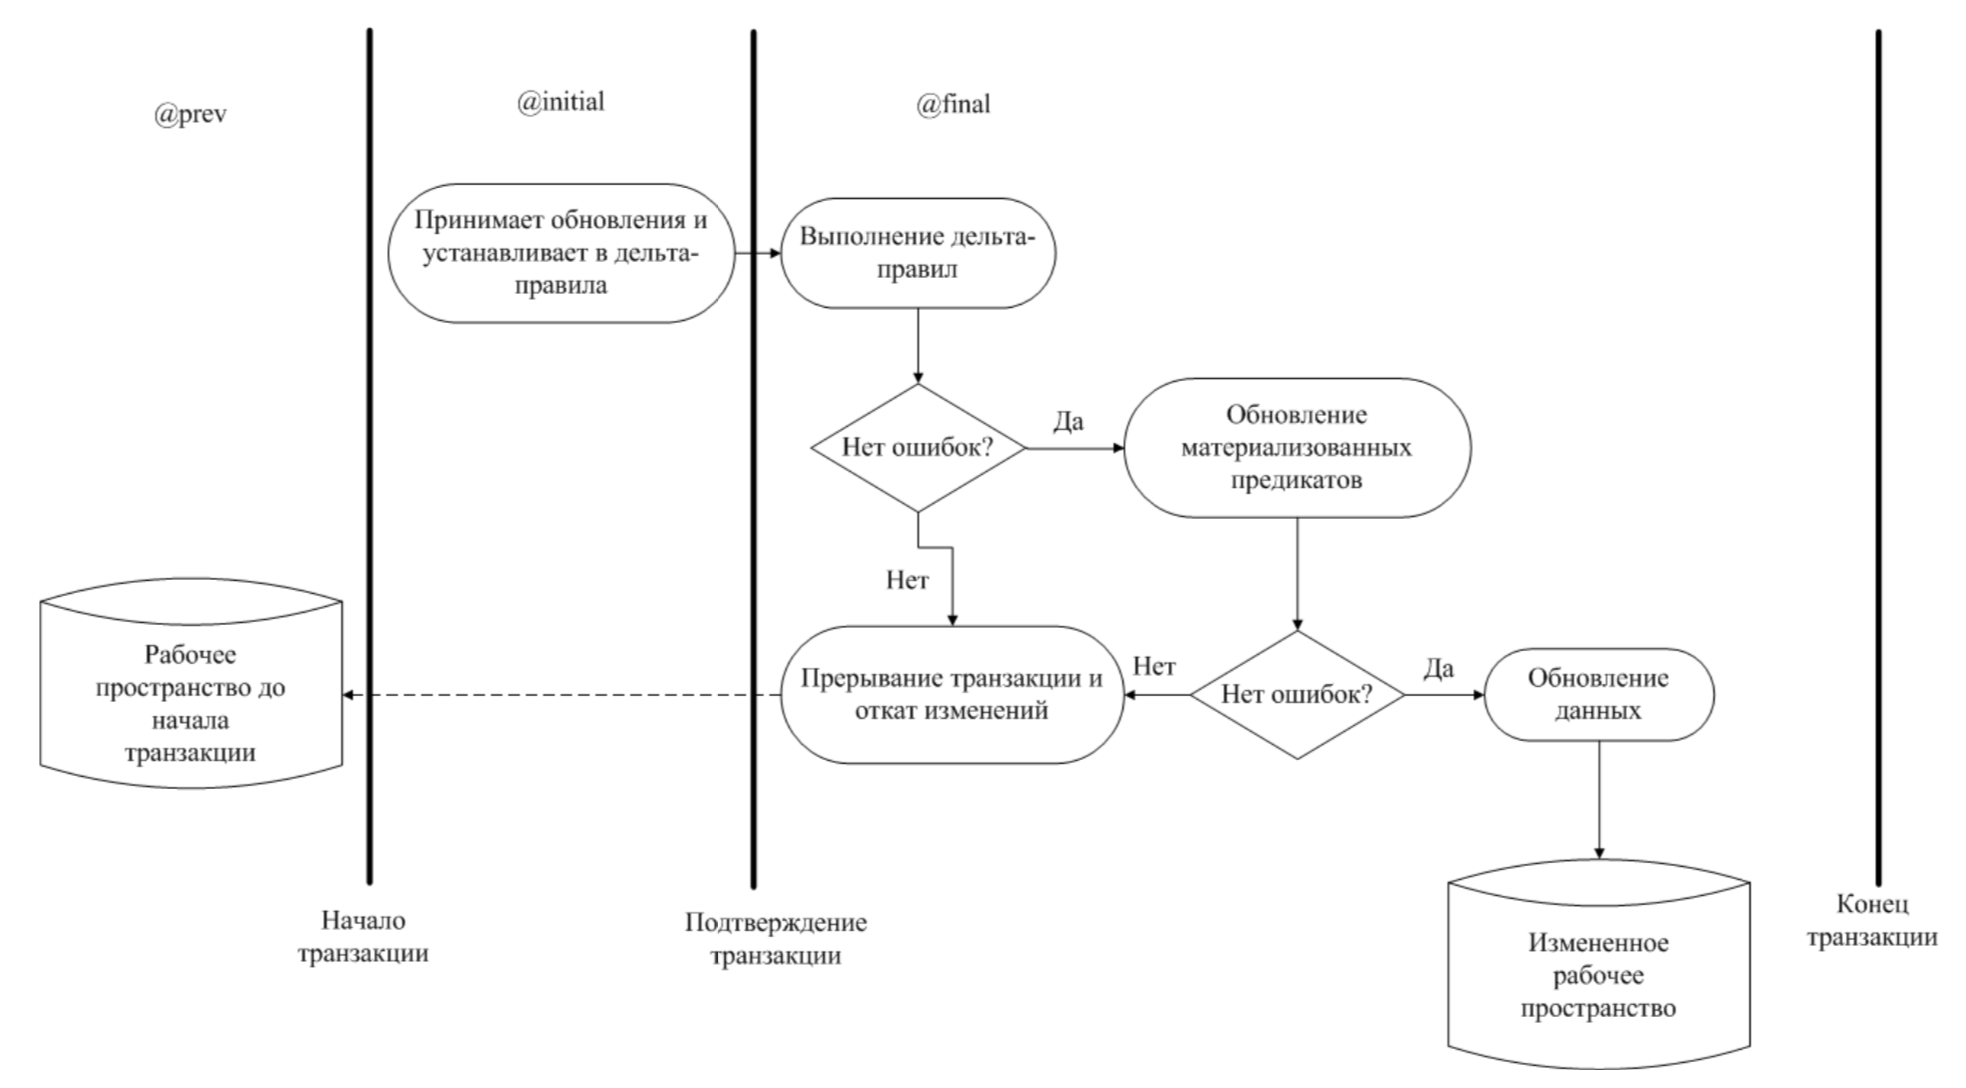
\includegraphics[scale=0.8]{transaction.png}
	\caption{Жизненный цикл транзакции}
	\label{fig:technology:logiql:transaction}
\end{figure}

\subsubsection{Бизнес-правила и агрегация}
\label{sec:technology:logiql:aggregations}

Теперь рассмотрим пример бизнес-правил в \logiql:

\begin{lstlisting}[language=Prolog]
netsales_u(product, store, day, net) <-
  sales_u(product, store, day, sls),
  returns_u(product, store, day, returns),
  net = sls - returns.

_(product, tunits) <-
  agg<< tunits=total(untis) >>
    sales_u(product, _, _, units).
\end{lstlisting}

Или, примерный аналог \sql:

\begin{lstlisting}[language=SQL]
CREATE VIEW netsales_u AS
SELECT DISTINCT S.product, S.store, S.day,
  S.unit – R.unit AS net
FROM sales_u S, returns_u R
WHERE S.product = R.product and
  S.store = R.store and
  S.day = R.day;
SELECT product, sum(units)
FROM unit_sales
GROUP BY product.
\end{lstlisting}

Здесь видно объявление еще одного предиката под названием \lstinline{netsales_u}, у которого 4 колонки и значение последней колонки вычисляется как разница значений из других предикатов. Опять же, если говорить в терминах языка \logiql, то определение будет звучать так: для всех записей с фиксированными \lstinline{product}, \lstinline{store}, \lstinline{day} в предикате \lstinline{sales_u} и записей для таких же \lstinline{product}, \lstinline{store}, \lstinline{day} в предикате \lstinline{returns_u} будет существовать запись в предикате \lstinline{netsales_u} с такими же \lstinline{product}, \lstinline{store}, \lstinline{day} и значением последней колонки, равной разнице между \lstinline{sls} и \lstinline{returns}. Другими словами, условие должно выполняться всегда, даже после обновления предикатов \lstinline{sales_u} и \lstinline{returns_u}, что гарантирует нам существование такой записи в \lstinline{netsales_u} \cite{query_language_for_smart_db}.

\subsubsection{Ограничения}
\label{sec:technology:logiql:constraints}

Попробуем наложить ограничения на значения в \logiql:

\begin{lstlisting}[language=Prolog]
sales_u[product, store, day] = unit ->
  string(product),
  string(store),
  datetime(day),
  int(unit).

sales_u[product, store, day] = unit ->
  product_catalog(product).

returns_u[product, store, day] = ret,
sales_u[product, store, day] = sls ->
  ret <= sls.
\end{lstlisting}

Или, аналог в \sql:

\begin{lstlisting}[language=SQL]
CREATE TABLE sales_u
(
  product VARCHAR(15) NOT NULL,
  store VARCHAR(20) NOT NULL,
  day DATETIME NOT NULL,
  unit INT NOT NULL,
  PRIMARY KEY (product, store, day),
  FOREIGN KEY (product)
    REFERENCES product_catalog(product)
);
\end{lstlisting}

В этом листинге появляется синтаксис с \lstinline{[...]}. Это определяет предикат типа ключ-значение. То, что находится в \lstinline{[]} является ключом, после знака равенства определяется значение. Вообще говоря, значение может быть не одно. В этом случае синтаксис немного изменится: \lstinline{some_predicate(key1, key2; val1, val2)}.

Фактически, \lstinline{sales_u} по-прежнему является предикатом с 4 колонками, но он функционально зависим. И если попытаться добавить еще одну запись с теми же \lstinline{product}, \lstinline{store}, \lstinline{day}, но с другим значением \lstinline{unit}, выбросится ошибка \lstinline{Constraint Violation}. Более того, такая нотация позволяет воспринимать этот предикат как функциональный, что при большом количестве предикатов в большом приложении упрощает задачу композиции различных предикатов. Итак, в примере указывается, что если в \lstinline{sales_u} имеется запись для некоторого \lstinline{product}, то такой \lstinline{product} должен находится в предикате \lstinline{product_catalog}. Аналогично, если для некоторых \lstinline{product}, \lstinline{store}, \lstinline{day} существуте запись в соответствующих предикатах,то обязательно должно выполняться \lstinline{ret <= sls}. Иначе, опять же, будет ошибка \lstinline{Constraint Violation}. Такие ограничения будут проверены каждый раз при обновлении записей в предикатах, причем лишь в тех, в которых это имеет смысл.
Среди преимуществ ограничений можно выделить следующие:
\begin{enumerate}
  \item Поддерживается подход «дизайн по контракту», согласно которому мы предполагаем, что ограничения выполняются всегда и нам не нужно их проверять самим. На выходе получаются более читабельные программы.
  \item Не позволяют пользователям выполнять операции, которые нарушают бизнес-правила.
  \item Автоматически расширяют предикаты для удовлетворения системы ограничений. Это ключ к интеграции с оптимизаторами.
\end{enumerate}

Рассмотрим еще один небольшой пример использования ограничений и покажем, насколько мощными они могут быть. Пусть существуют следующие предикаты:

\begin{lstlisting}[language=Prolog]
node(n), node_id(n:uuid) -> string(uuid).
color(c), color(c:color_name) -> string(color_name). edge(u, v) -> node(u), node(v).
color_of[n] = c -> node(n), color(c).
node(n) -> color_of[n] = _.
edge(x, y), color_of[x] = c, color_of[y] = c -> x = y.
\end{lstlisting}

Здесь указаны необходимые предикаты для вершины, ребра и цвета вершины графа. Кроме того, наложено ограничения о том, что каждая вершина должна иметь некоторый цвет и никакие две смежные вершины не могут иметь одинаковый цвет. А теперь с помощью \LB это легко подключается к оптимизатору (например, \emph{Gurobi}), который может найти минимальную возможную раскраску графа. Это достигается лишь одной строкой:

\begin{lstlisting}[language=Prolog]
lang:solver:variable(`color_of).
\end{lstlisting}

Этот пример показывает простую связь между декларативным программированием и программированием в ограничениях \cite{logiql_vs_datalog}.

\subsubsection{Триггеры, события}
\label{sec:technology:logiql:triggers_events}

Рассмотрим триггеры и события на языке \logiql.

\begin{lstlisting}[language=Prolog]
^sales_u[product, store, day] = new_units <-
  +sales_line[_, product, store, day] = line_untis,
  sales_u@prev[product, store, day] = units,
  new_units = line_units + units.
\end{lstlisting}

Или, аналог в \sql:

\begin{lstlisting}[language=SQL]
CREATE TRIGGER update_sales ON sales_line
AFTER INSERT BEGIN
UPDATE sales_u
SET sales_u.units = inserted.units + sales_u.units
FROM sales_u, inserted
WHERE sales_u.product = inserted.product and
  sales_u.store = inserted.store and
  sales_u.day = inserted.day
END;
\end{lstlisting}

Приведенный листинг явно показывает краткость записи в \logiql. Данное правило при каждом добавлении записи в \lstinline{sales_line} при выполнении указанного условия будет обновлять значение в предикате \lstinline{sales_u}. Здесь используется так называемое «дельта правило» (со знаком «\lstinline{+}» и «\lstinline{^}»), которое в данном случае говорит о вставке записи. Так же существует дельта правила на обновление (\lstinline{upsert}) и удаление. \lstinline{@prev} здесь указывает на одну стадию жизненного цикла транзакции (в конкретном случае – до начала транзакции).
Единственные отрицательные стороны данного (по сравнению с \sql) подхода в том, что события не могут вызывать другие события и события также не могут изменять схему \cite{query_language_for_smart_db}.

\subsubsection{Queries и Spreads}
\label{sec:technology:logiql:queries_spreads}

В \logiql все запросы разделяются на \emph{queries} и \emph{spreads}. Первые используются для получения информации (значений предикатов, агрегированной информации), вторые – для обновления информации. Пример из главы про бизнес-правила является типичным примером \emph{query}, где может происходить выборка по количеству проданных продуктов, а пример из предыдущей главы служит как \emph{spread} – с помощью него можно обновлять значения в предикатах при изменении в других.
Видно наглядно, что на языке \logiql описание предикатов и правил смотрятся логичнее, проще и понятнее, чем в \sql. Эта лаконичность также является одной из особенностей этого языка.
Выделим ключевые моменты языка \logiql:

\begin{enumerate}
  \item декларативный язык;
  \begin{itemize}
    \item нормализация ключ-значение (6 нормальная форма);
    \item булева логика  не содержит нулевых записей;
    \item семантика множеств;
  \end{itemize}
  \item выразительный;
  \begin{itemize}
    \item правила/запросы аналогичны \sql views и запросам;
    \item событийные правила с той же смысловой нагрузкой, что и в \sql, но проще в реализации;
    \item делает возможным оптимизации, машинное обучение легковстраиваевым \cite{query_language_for_smart_db}.
  \end{itemize}
\end{enumerate}
